\documentclass[tikz,border=10pt]{standalone}
\usepackage{amsmath}
\usetikzlibrary{arrows.meta,calc,positioning}
\definecolor{partblue}{HTML}{0072B2}
\definecolor{partgreen}{HTML}{009E73}
\definecolor{partorange}{HTML}{E69F00}
\definecolor{partpurple}{HTML}{CC79A7}
\definecolor{partred}{HTML}{D55E00}
\definecolor{ink}{HTML}{25334A}
\begin{document}
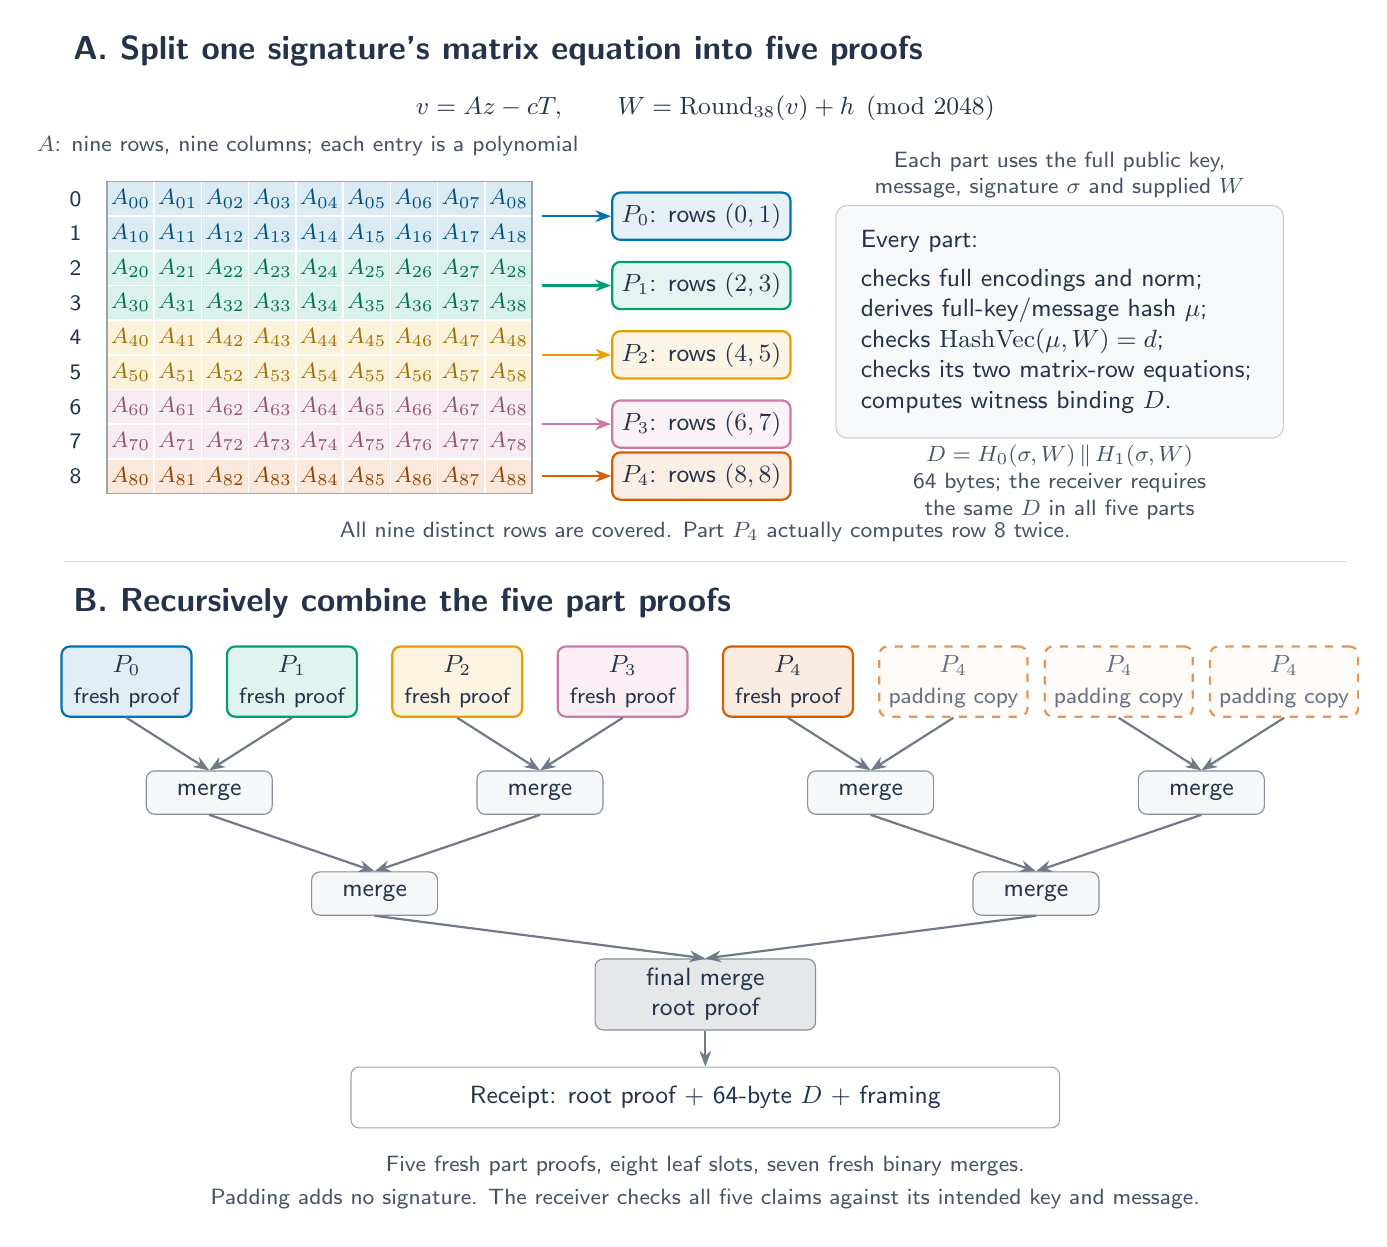
\begin{tikzpicture}[font=\sffamily\small,text=ink,
 arrow/.style={-{Stealth[length=2mm]},line width=.8pt,draw=ink!65},
 part/.style={rounded corners=3pt,draw,line width=.8pt,minimum width=2.15cm,minimum height=.60cm,align=center},
 leaf/.style={part,minimum width=1.65cm,minimum height=.75cm},
 merge/.style={rounded corners=3pt,draw=ink!55,fill=ink!4,minimum width=1.6cm,minimum height=.55cm,align=center},
 note/.style={font=\sffamily\footnotesize,align=center,text=ink!85}]

\node[anchor=west,font=\sffamily\bfseries\large] at (0,0) {A. Split one signature's matrix equation into five proofs};
\node at (8.15,-.72) {$v=Az-cT,\qquad W=\operatorname{Round}_{38}(v)+h\pmod{2048}$};
\node[note] at (3.1,-1.2) {$A$: nine rows, nine columns; each entry is a polynomial};

\foreach \r in {0,...,8} {
  \ifnum\r<2 \def\rowcolor{partblue}\else
  \ifnum\r<4 \def\rowcolor{partgreen}\else
  \ifnum\r<6 \def\rowcolor{partorange}\else
  \ifnum\r<8 \def\rowcolor{partpurple}\else
  \def\rowcolor{partred}\fi\fi\fi\fi
  \pgfmathsetmacro{\yc}{-1.65-.44*\r}
  \node[anchor=east,font=\sffamily\footnotesize] at (.35,\yc-.22) {\r};
  \foreach \j in {0,...,8} {
    \pgfmathsetmacro{\xc}{.55+.60*\j}
    \path[fill=\rowcolor!14,draw=white,line width=.6pt] (\xc,\yc) rectangle ++(.60,-.44);
    \node[font=\footnotesize,text=\rowcolor!70!black] at (\xc+.30,\yc-.22) {$A_{\r\j}$};
  }
}
\draw[ink!45,line width=.5pt] (.55,-1.65) rectangle (5.95,-5.61);
\foreach \p/\ya/\ra/\rb/\col in {0/-2.09/0/1/partblue,1/-2.97/2/3/partgreen,2/-3.85/4/5/partorange,3/-4.73/6/7/partpurple,4/-5.39/8/8/partred} {
  \node[part,draw=\col,fill=\col!10] (P\p) at (8.1,\ya) {$P_{\p}$: rows $(\ra,\rb)$};
  \draw[arrow,draw=\col] (6.08,\ya) -- (P\p.west);
}
\node[note,text width=5.2cm] at (12.65,-1.57) {Each part uses the full public key,\\message, signature $\sigma$ and supplied $W$};
\node[draw=ink!25,fill=ink!3,rounded corners=4pt,align=left,text width=5.05cm,inner sep=9pt] at (12.65,-3.43) {Every part:\\[3pt]
  checks full encodings and norm;\\
  derives full-key/message hash $\mu$;\\
  checks $\operatorname{HashVec}(\mu,W)=d$;\\
  checks its two matrix-row equations;\\
  computes witness binding $D$.};
\node[note] at (12.65,-5.13) {$D=H_0(\sigma,W)\,\|\,H_1(\sigma,W)$};
\node[note] at (12.65,-5.65) {64 bytes; the receiver requires\\the same $D$ in all five parts};
\node[note] at (8.15,-6.10) {All nine distinct rows are covered. Part $P_4$ actually computes row 8 twice.};

\draw[ink!15] (0,-6.48) -- (16.3,-6.48);
\node[anchor=west,font=\sffamily\bfseries\large] at (0,-7.00) {B. Recursively combine the five part proofs};

\foreach \p/\col in {0/partblue,1/partgreen,2/partorange,3/partpurple,4/partred} {
 \pgfmathsetmacro{\xp}{.8+2.1*\p}
 \node[leaf,draw=\col,fill=\col!12] (L\p) at (\xp,-8.00) {$P_{\p}$\\\footnotesize fresh proof};
}
\foreach \p in {5,6,7} {
 \pgfmathsetmacro{\xp}{.8+2.1*\p}
 \node[leaf,draw=partred!65,dashed,fill=partred!3,text=ink!70] (L\p) at (\xp,-8.00) {$P_4$\\\footnotesize padding copy};
}
\foreach \p/\a/\b in {0/0/1,1/2/3,2/4/5,3/6/7} {
 \node[merge] (M\p) at ($(L\a.south)!.5!(L\b.south)+(0,-.95)$) {merge};
 \draw[arrow] (L\a.south) -- (M\p.north);
 \draw[arrow] (L\b.south) -- (M\p.north);
}
\foreach \p/\a/\b in {0/0/1,1/2/3} {
 \node[merge] (N\p) at ($(M\a.south)!.5!(M\b.south)+(0,-1.00)$) {merge};
 \draw[arrow] (M\a.south) -- (N\p.north);
 \draw[arrow] (M\b.south) -- (N\p.north);
}
\node[merge,fill=ink!12,minimum width=2.8cm,minimum height=.75cm] (Root) at ($(N0.south)!.5!(N1.south)+(0,-1.00)$) {final merge\\root proof};
\draw[arrow] (N0.south) -- (Root.north);
\draw[arrow] (N1.south) -- (Root.north);
\node[draw=ink!45,rounded corners=3pt,align=center,inner sep=7pt,minimum width=9cm] (Receipt) at ($(Root.south)+(0,-.85)$) {Receipt: root proof + 64-byte $D$ + framing};
\draw[arrow] (Root.south) -- (Receipt.north);
\node[note] at ($(Receipt.south)+(0,-.48)$) {Five fresh part proofs, eight leaf slots, seven fresh binary merges.};
\node[note] at ($(Receipt.south)+(0,-.90)$) {Padding adds no signature. The receiver checks all five claims against its intended key and message.};
\end{tikzpicture}
\end{document}
